\documentclass[aspectratio=43]{beamer}

\usepackage[T1]{fontenc}
\usepackage[utf8]{inputenc}
\usepackage[english]{babel}
\usepackage{lmodern}
\usepackage{booktabs}


%import the theme and packages for the code blocks
\usepackage{listings}
\usepackage{xcolor}

% Definizione colori
\definecolor{sfondo}{RGB}{245,245,245}
\definecolor{bordo}{RGB}{180,180,180}
\definecolor{codice}{RGB}{20,20,120}
\definecolor{commento}{RGB}{100,100,100}
\definecolor{stringa}{RGB}{180,0,0}
\definecolor{parolaChiave}{RGB}{0,0,180}

% Stile personalizzato
\lstset{
	language=R,
	backgroundcolor=\color{sfondo},
	frame=single,
	rulecolor=\color{bordo},
	basicstyle=\ttfamily\small\color{codice},
	keywordstyle=\color{parolaChiave}\bfseries,
	commentstyle=\color{commento}\itshape,
	stringstyle=\color{stringa},
	numbers=left,
	numberstyle=\tiny\color{gray},
	numbersep=5pt,
	showstringspaces=false,
	breaklines=true,
	emph={saluta,print,paste}, % parole da evidenziare
	emphstyle=\color{magenta}
}


% Use Unipd as theme, with options:
% - pageofpages: define the separation symbol of the footer page of pages (e.g.: of, di, /, default: of)
% - logo: position another logo near the Unipd logo in the title page (e.g. department logo), passing the second logo path as option 
% Use the environment lastframe to add the endframe text
\usetheme[pageofpages=of]{Unipd}

\title{Temporal and spatial analysis of earthquakes in Italy in the last century\\}
\subtitle{}
\author[]{Jamilov Javlon, Pirazzo Tommaso, Secco Benedetto}

\date{14 luglio 2025}


\begin{document}

% Make the title page
\frame{\titlepage}

%--------------------------------------------------------------- project part
\section{Introduction}

\begin{frame}{What is this project about?}
	In this work we studied the temporal and spatial analysis of earthquakes in Italy in the period 1925-2025. 
	To achieve the goal of giving a complete and exhaustive picture of the phenomenon, we followed the following steps:\pause
	
	\vspace*{1cm}
	
	\begin{enumerate}
		\item Prepare and inspect the data;\pause
			\vspace*{0.5cm}
		\item Spatial anlysis (Hazard map and hierarchical clustering);\pause
			\vspace*{0.5cm}
		\item Sviluppo (Forecast with ARIMA and SSA model);\pause
	\end{enumerate}
\end{frame}

%This is simply an example of how to start the presentation...you can change as you desire
\begin{frame}{What is this project about?}
	\begin{figure}[h]
		\centering
		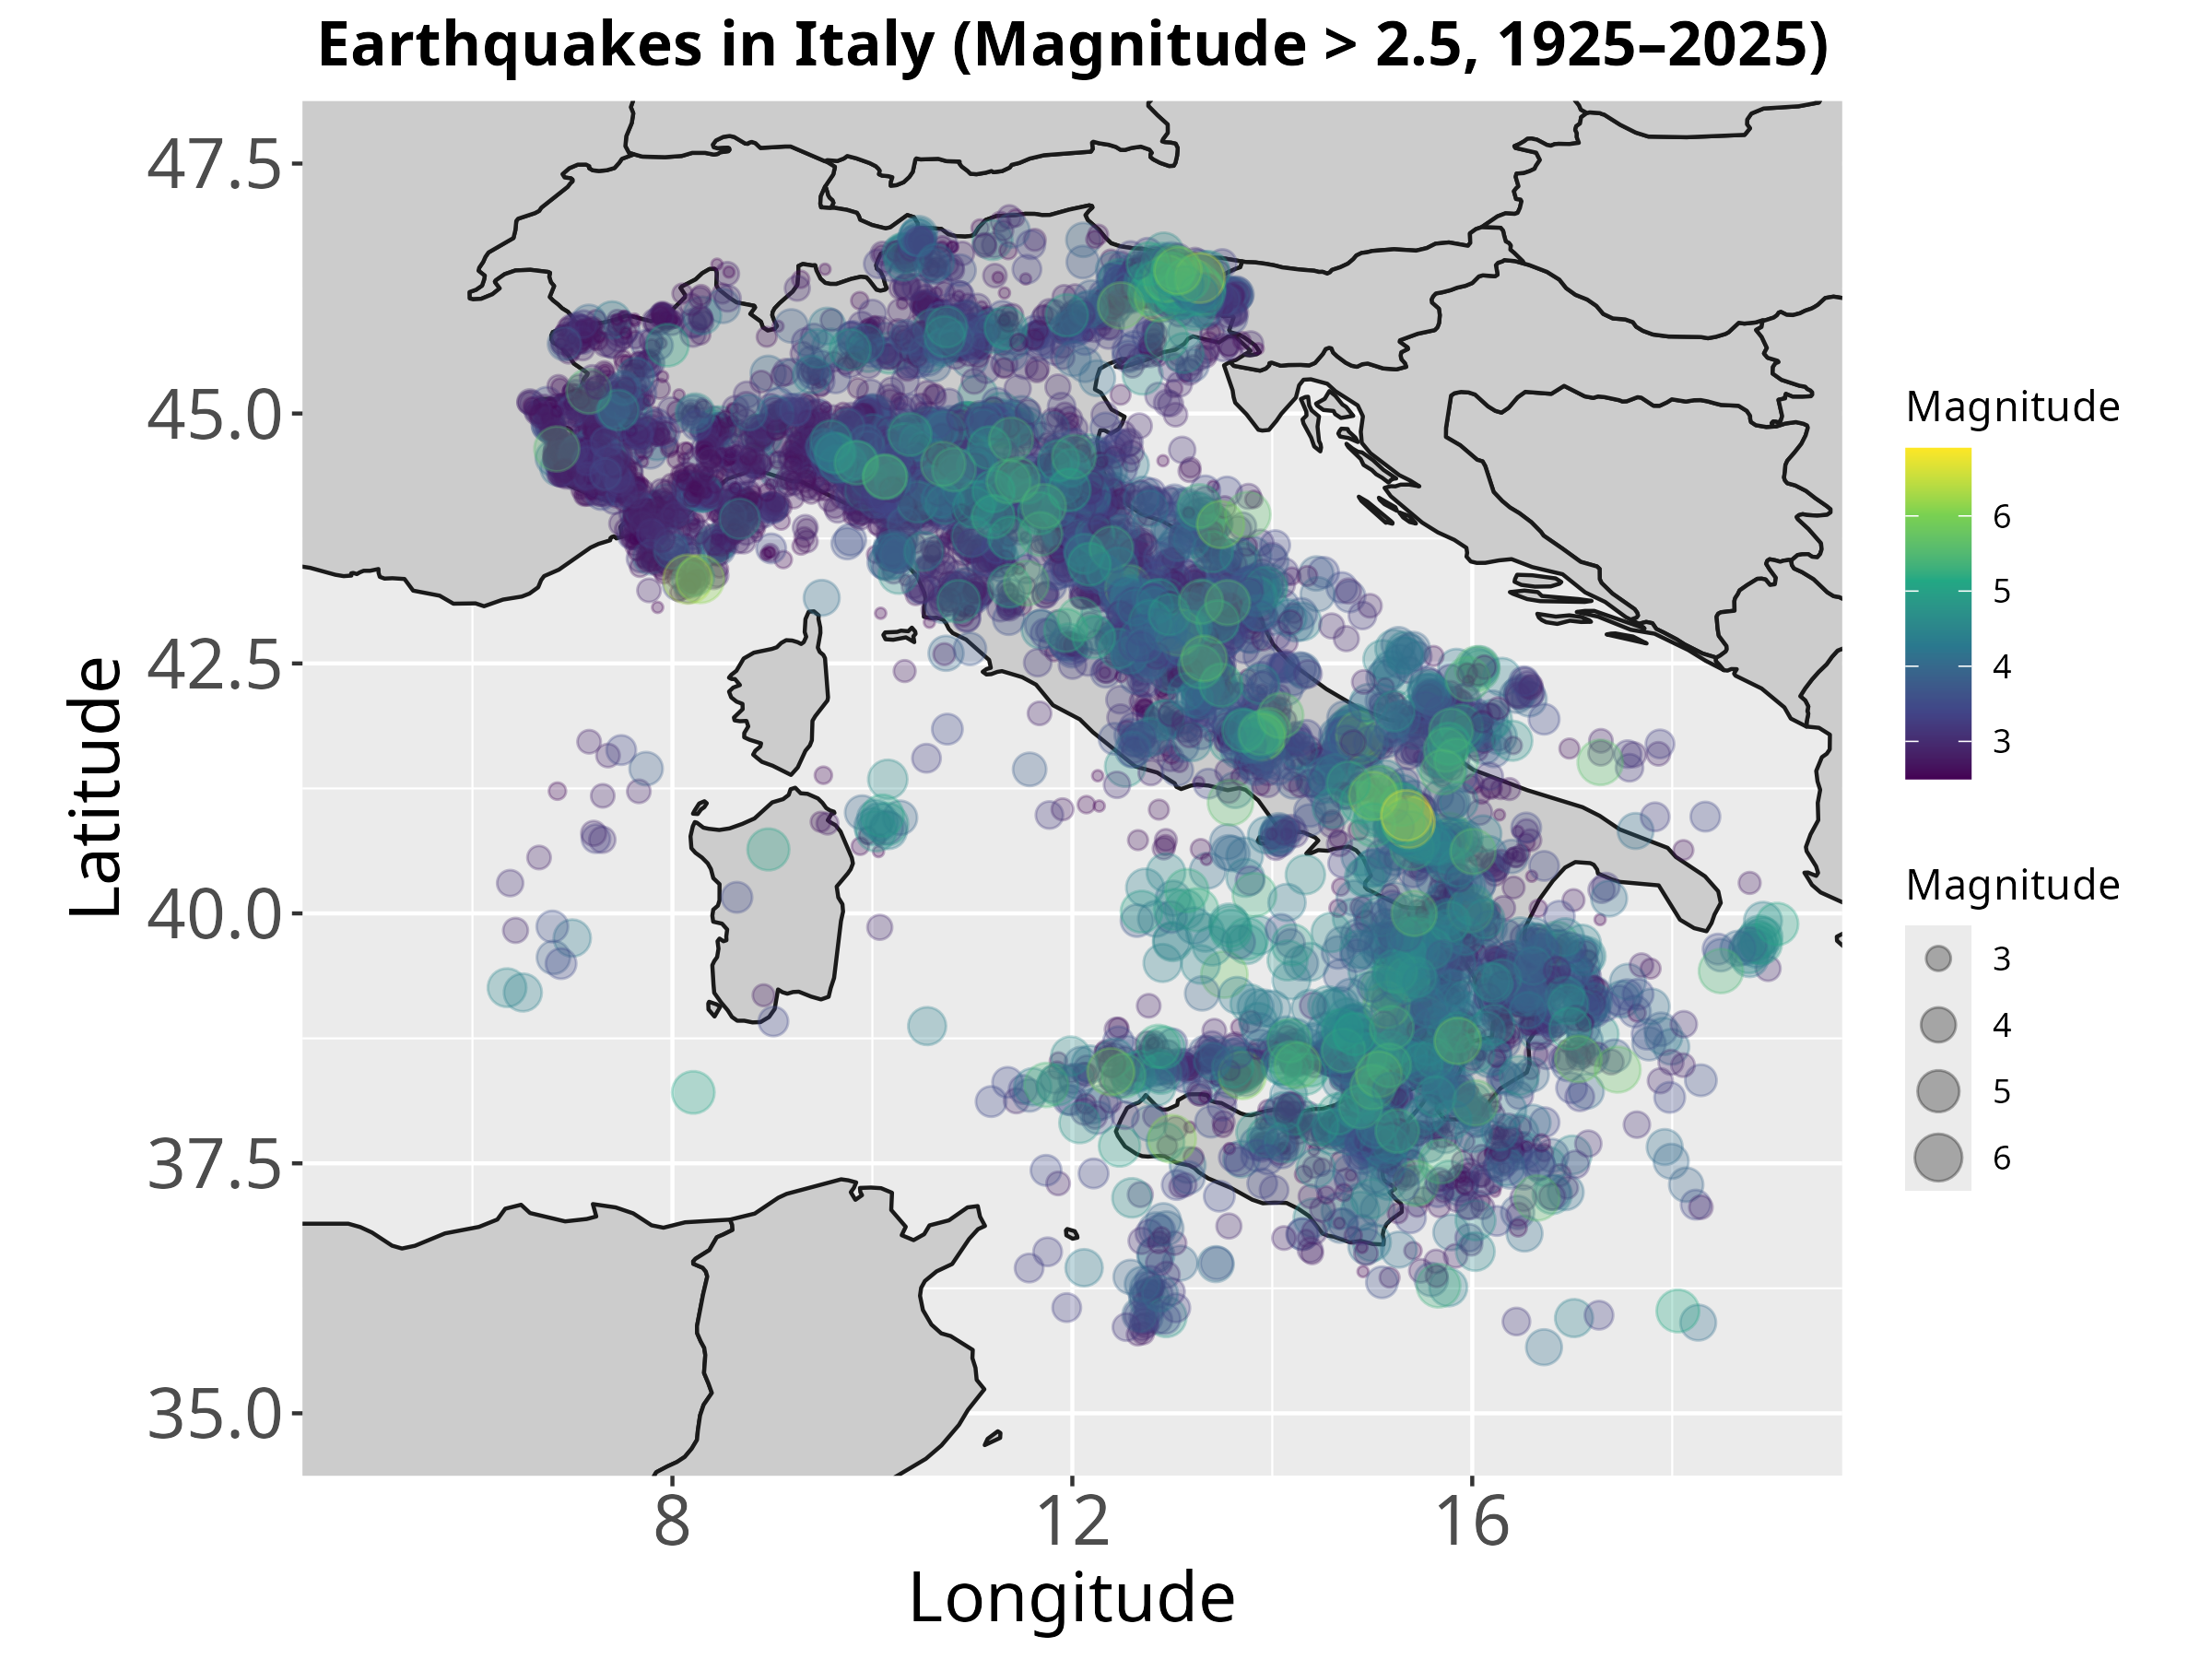
\includegraphics[width=0.95\textwidth]{EQ_images/all_earthquakes.png}
	\end{figure}
\end{frame}


\section{First Part}

\begin{frame}{Focus on high magnitude events}
	\begin{figure}[h]
		\centering
		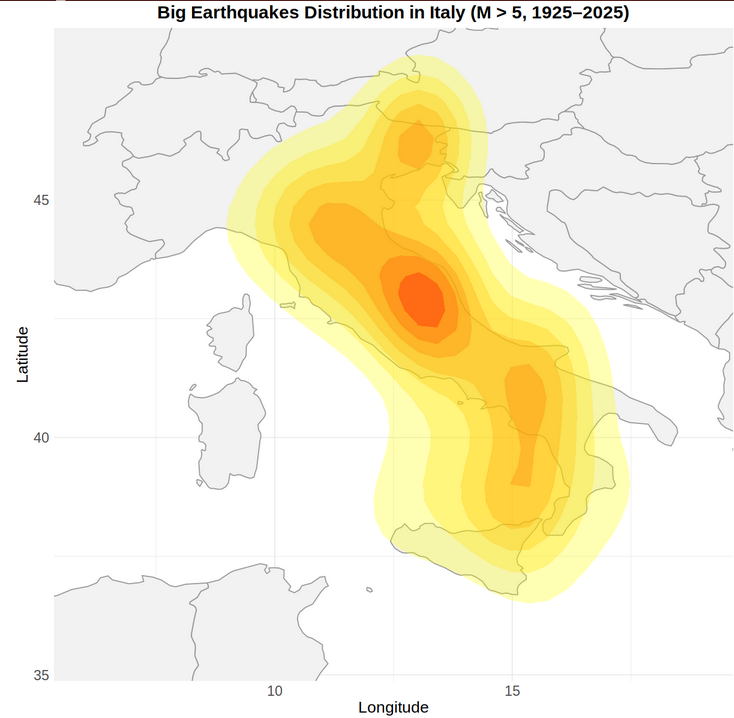
\includegraphics[width=0.75\textwidth]{EQ_images_ben/eq_density_map.png}
	\end{figure}
\end{frame}

\begin{frame}{Focus on high magnitude events}
	\begin{figure}[h]
		\centering
		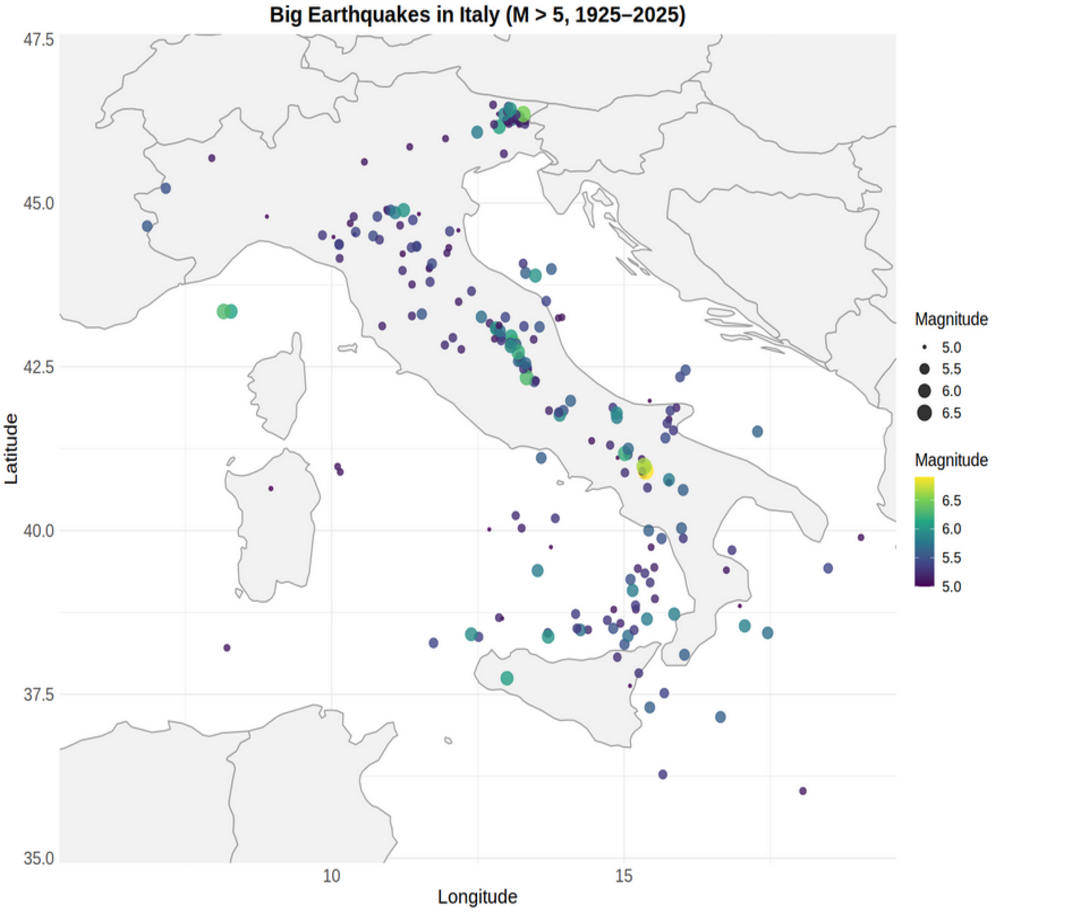
\includegraphics[width=0.85\textwidth]{EQ_images_ben/eq_map_italy.png}
	\end{figure}
\end{frame}

\begin{frame}{Focus on high magnitude events}
	\begin{figure}[t]
		\centering
		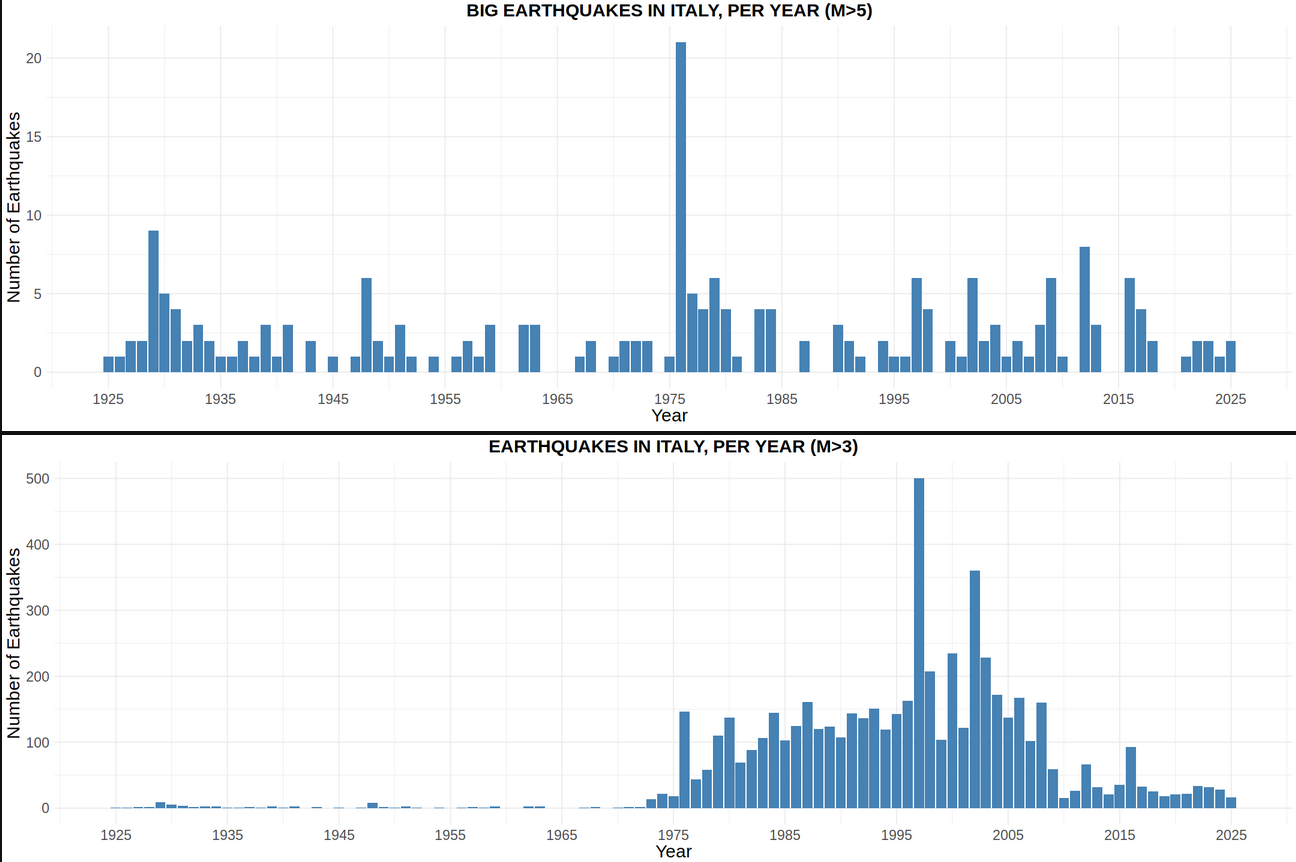
\includegraphics[width=0.75\textwidth]{EQ_images_ben/eq_hist_years.png}
	\end{figure}
	
	\pause
	
	Bad technology.... %TODO
\end{frame}


\begin{frame}{Seasonality?}
	\begin{figure}[t]
		\centering
		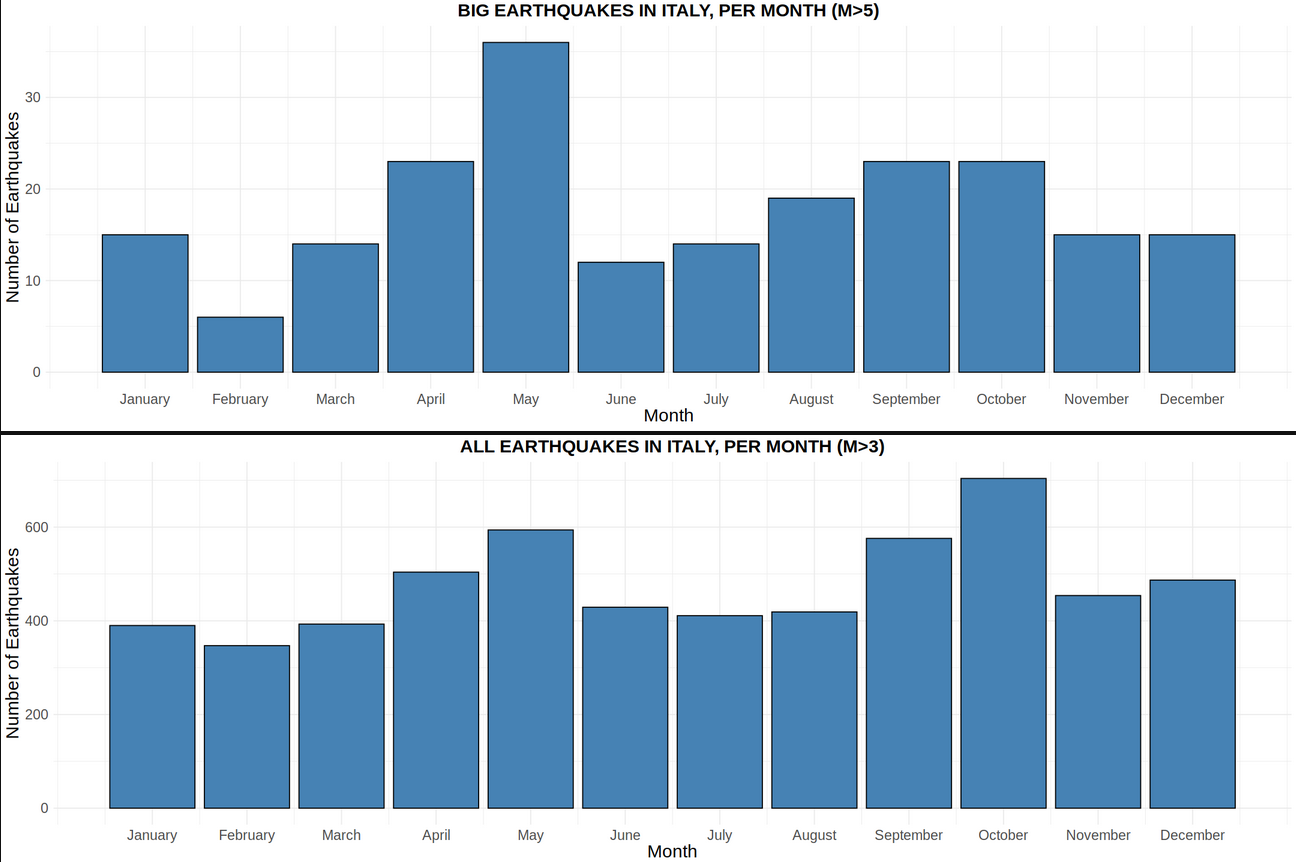
\includegraphics[width=0.85\textwidth]{EQ_images_ben/eq_hist_months.png}
	\end{figure}
	
\end{frame}

\begin{frame}{Depth histograms}
	\begin{figure}[t]
		\centering
		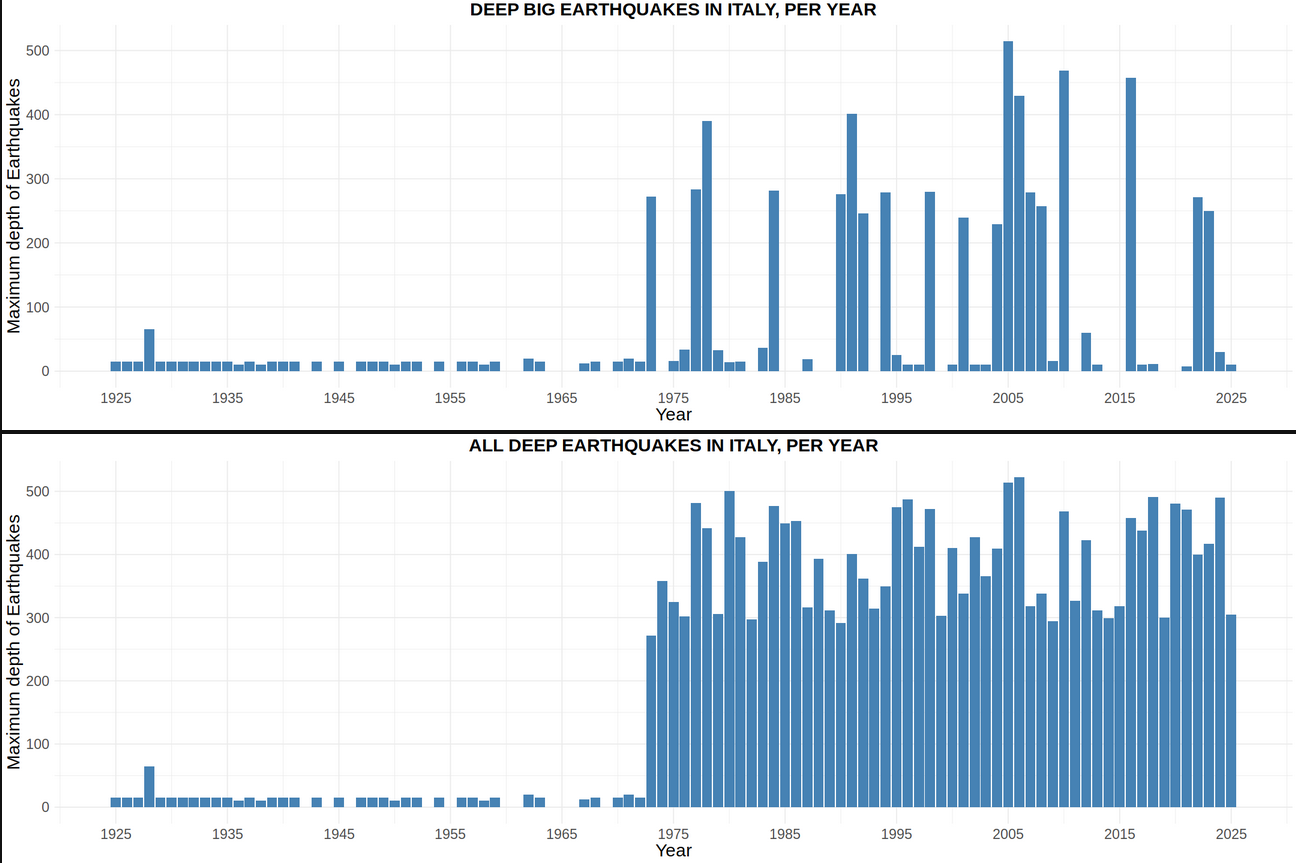
\includegraphics[width=0.85\textwidth]{EQ_images_ben/eq_hist_depth_years.png}
	\end{figure}
\end{frame}

\begin{frame}{Depth histograms}
	\begin{figure}[t]
		\centering
		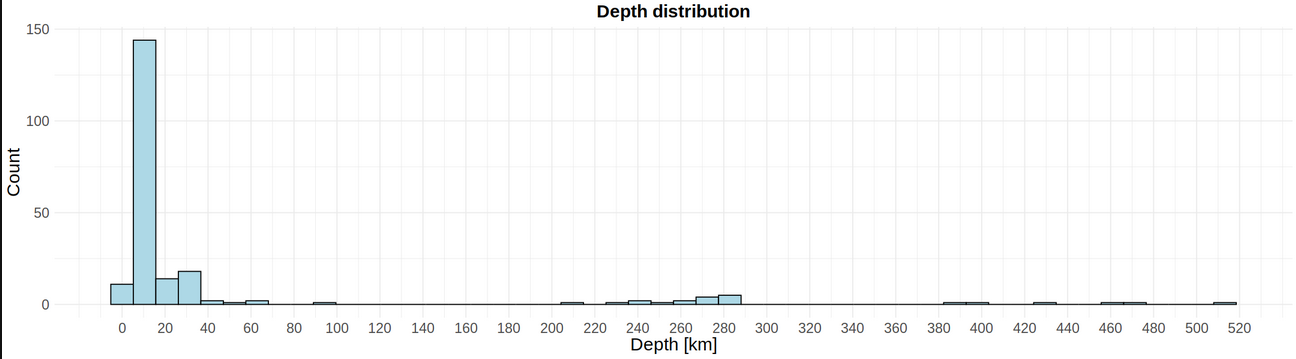
\includegraphics[width=1\textwidth]{EQ_images_ben/eq_hist_depth.png}
	\end{figure}
	
	From the histogram we can identify three main depth zones: \pause
	\begin{itemize} 
		\item $0-40 \ km$ \pause
		\item $230-290 \ km$ \pause
		\item $> 350 \ km$ 
	\end{itemize}	
\end{frame}


\begin{frame}{Depth map}
	
\begin{columns}
	
	\begin{column}{0.8\textwidth}
		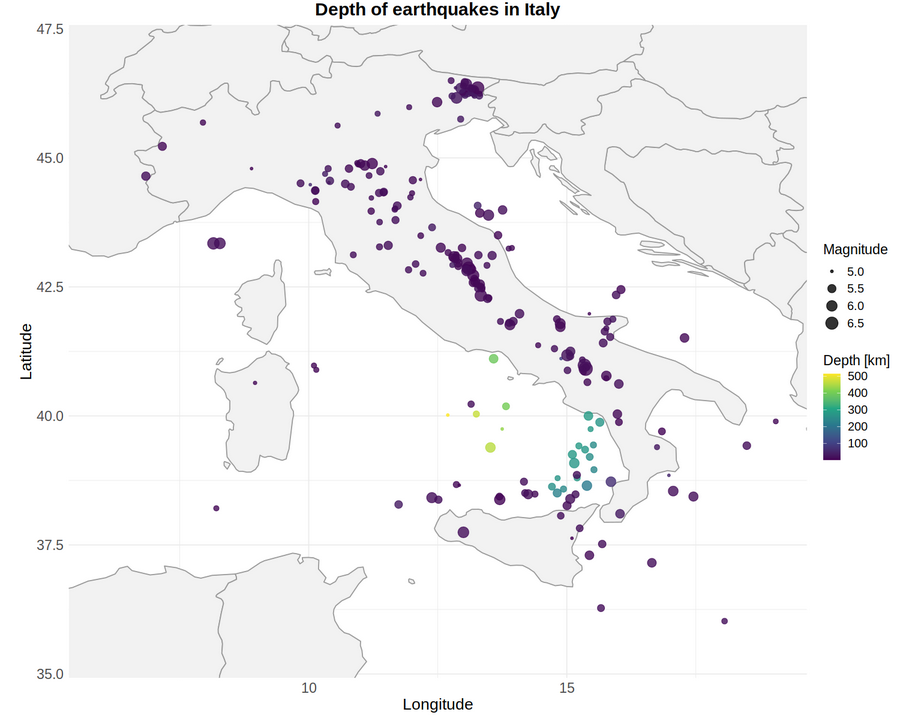
\includegraphics[width=1\textwidth]{EQ_images_ben/eq_depth_map.png}
	\end{column}
	
	\begin{column}{0.6\textwidth}
		\begin{itemize}
			\item Primo punto
			\item Secondo punto
			\item Terzo punto
		\end{itemize}
	\end{column}
	
\end{columns}
	
\end{frame}



\begin{frame}{Variables correlation}
	\begin{figure}[t]
		\centering
		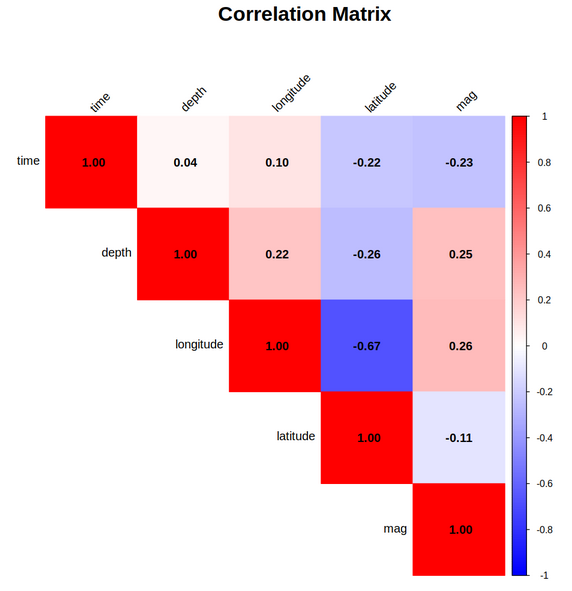
\includegraphics[width=0.77\textheight]{EQ_images_ben/eq_correlation_matrix.png}
	\end{figure}	
\end{frame}

\begin{frame}{Variables correlation}
	\begin{figure}[t]
		\centering
		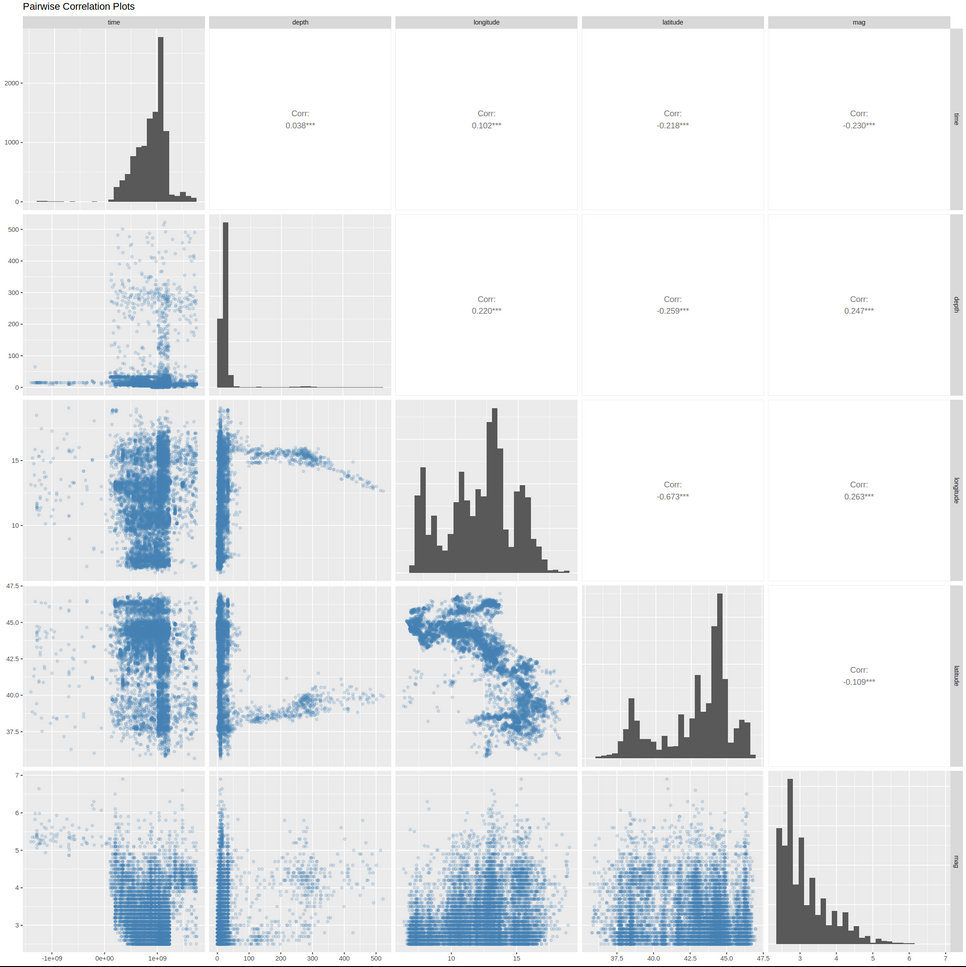
\includegraphics[width=0.77\textheight]{EQ_images_ben/eq_correlation_plots.png}
	\end{figure}	
\end{frame}


\begin{frame}{The Gutenbergh-Richter Law}
	
	\begin{figure}[t]
		\centering
		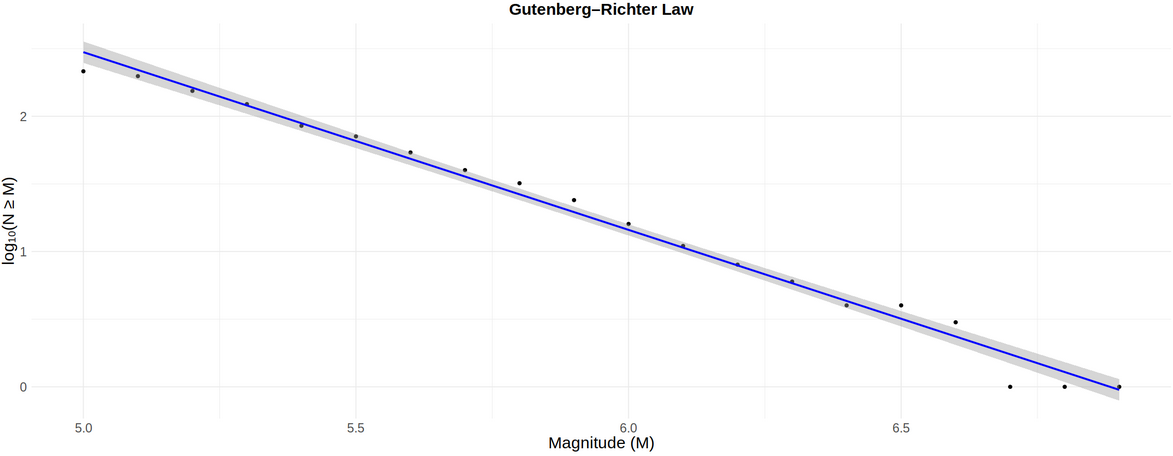
\includegraphics[width=1\textwidth]{EQ_images_ben/eq_gr_law.png}		
	\end{figure}
	

		\centering
		\begin{tabular}{c|ccc}
			\toprule
			    & Value & Error & $\chi^2$ \\
			    & units & units & \\
			\midrule
			a & ... & ... & \\
			b  & ... & ... & \\
			\bottomrule
		\end{tabular}
		
\end{frame}


\section{Second Part}

\begin{frame}{Spatial analysis}

In order to obtain a sismic map based on the Gutemberg-Richter law We followed these steps:\pause

\begin{enumerate}
	\item Divide the Region into grid Cells; \pause
	\item Count the number of events above magnitude $4$ (Trade-off); \pause
	\item Fit the G-R law using linear regression on $log_{10}(N)$ vs. $M$; \pause
	\item Derive local $a$ and $b$ values; \pause
	
\end{enumerate}

\centering
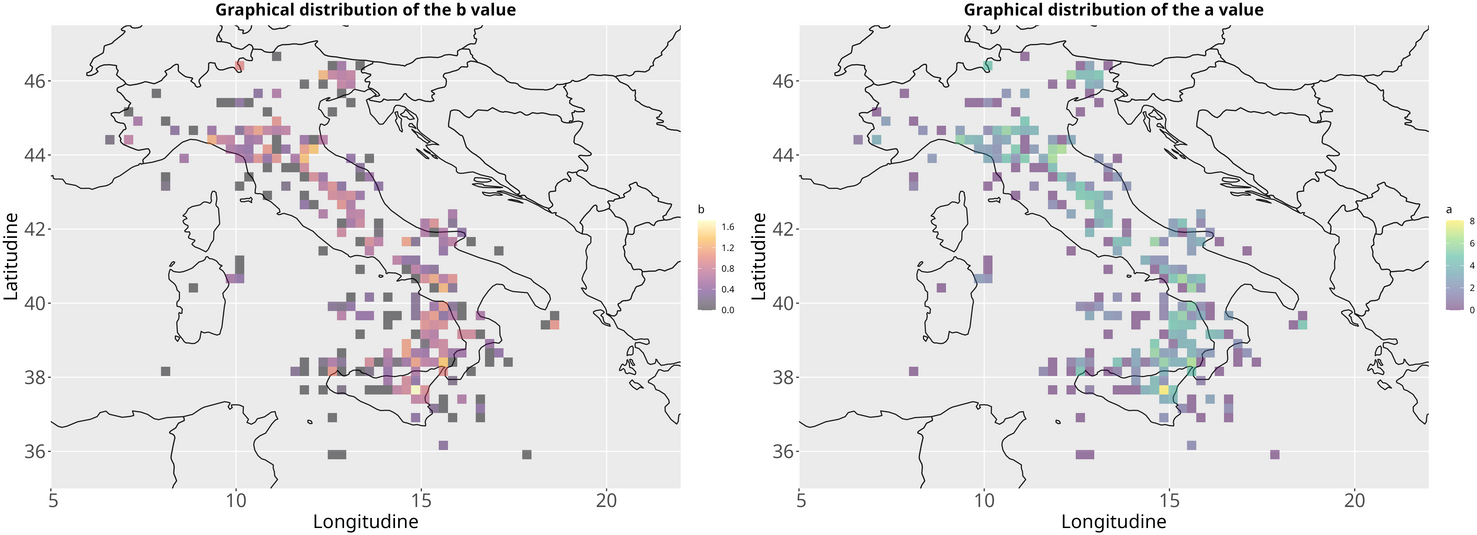
\includegraphics[width=1\textwidth]{EQ_images/G_R_parameters.png} \\

\end{frame}

	
\begin{frame}[fragile]{Adding tectonic plates boundaries}
	\begin{lstlisting}[language=R, basicstyle=\ttfamily\scriptsize]
# https://www.usgs.gov/programs/earthquake-hazards/google-earthtmkml-files -> page where you can find the file for the edge of the plates
		
plates <- st_read("doc.kml", layer = "Plate Interface")
		...
		
# add tectonic plates boundaries
a_plot_plates <- ggplot() +

	# borders
	borders("world", 
	regions = c(reg), 
	fill = "gray80", colour = "gray10", alpha = 0) +
			
	# tectonic plates boundaries layer
	geom_sf(data = plates, color = "blue", size = 2) +
		...
	\end{lstlisting}
\end{frame}
	

\begin{frame}{Adding tectonic plates boundaries}
	%aggiungere codice placche
	\centering
	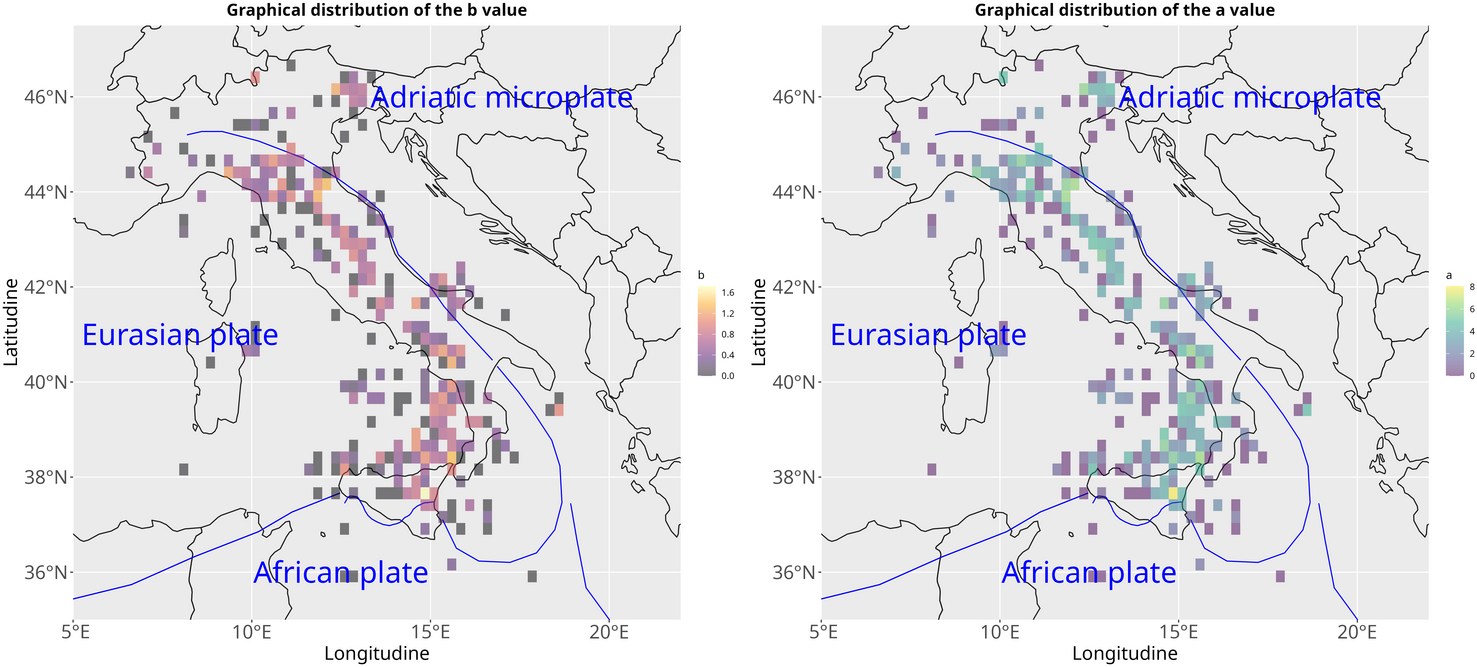
\includegraphics[width=1\textwidth]{EQ_images/G_R_parameters_plates.png} \\
\end{frame}

\begin{frame}{Naive model for sismic hazard}
	%aggiungere codice placche
	\centering
	In order to provide an exstimation of the sismic hazard in Italy, We tried to calculate the probability to have at least 1 high magnitude event in the next 10 years assuming that the intense events follw a Poisson distribution.  
\end{frame}

\begin{frame}{Naive model for sismic hazard}
	\centering
	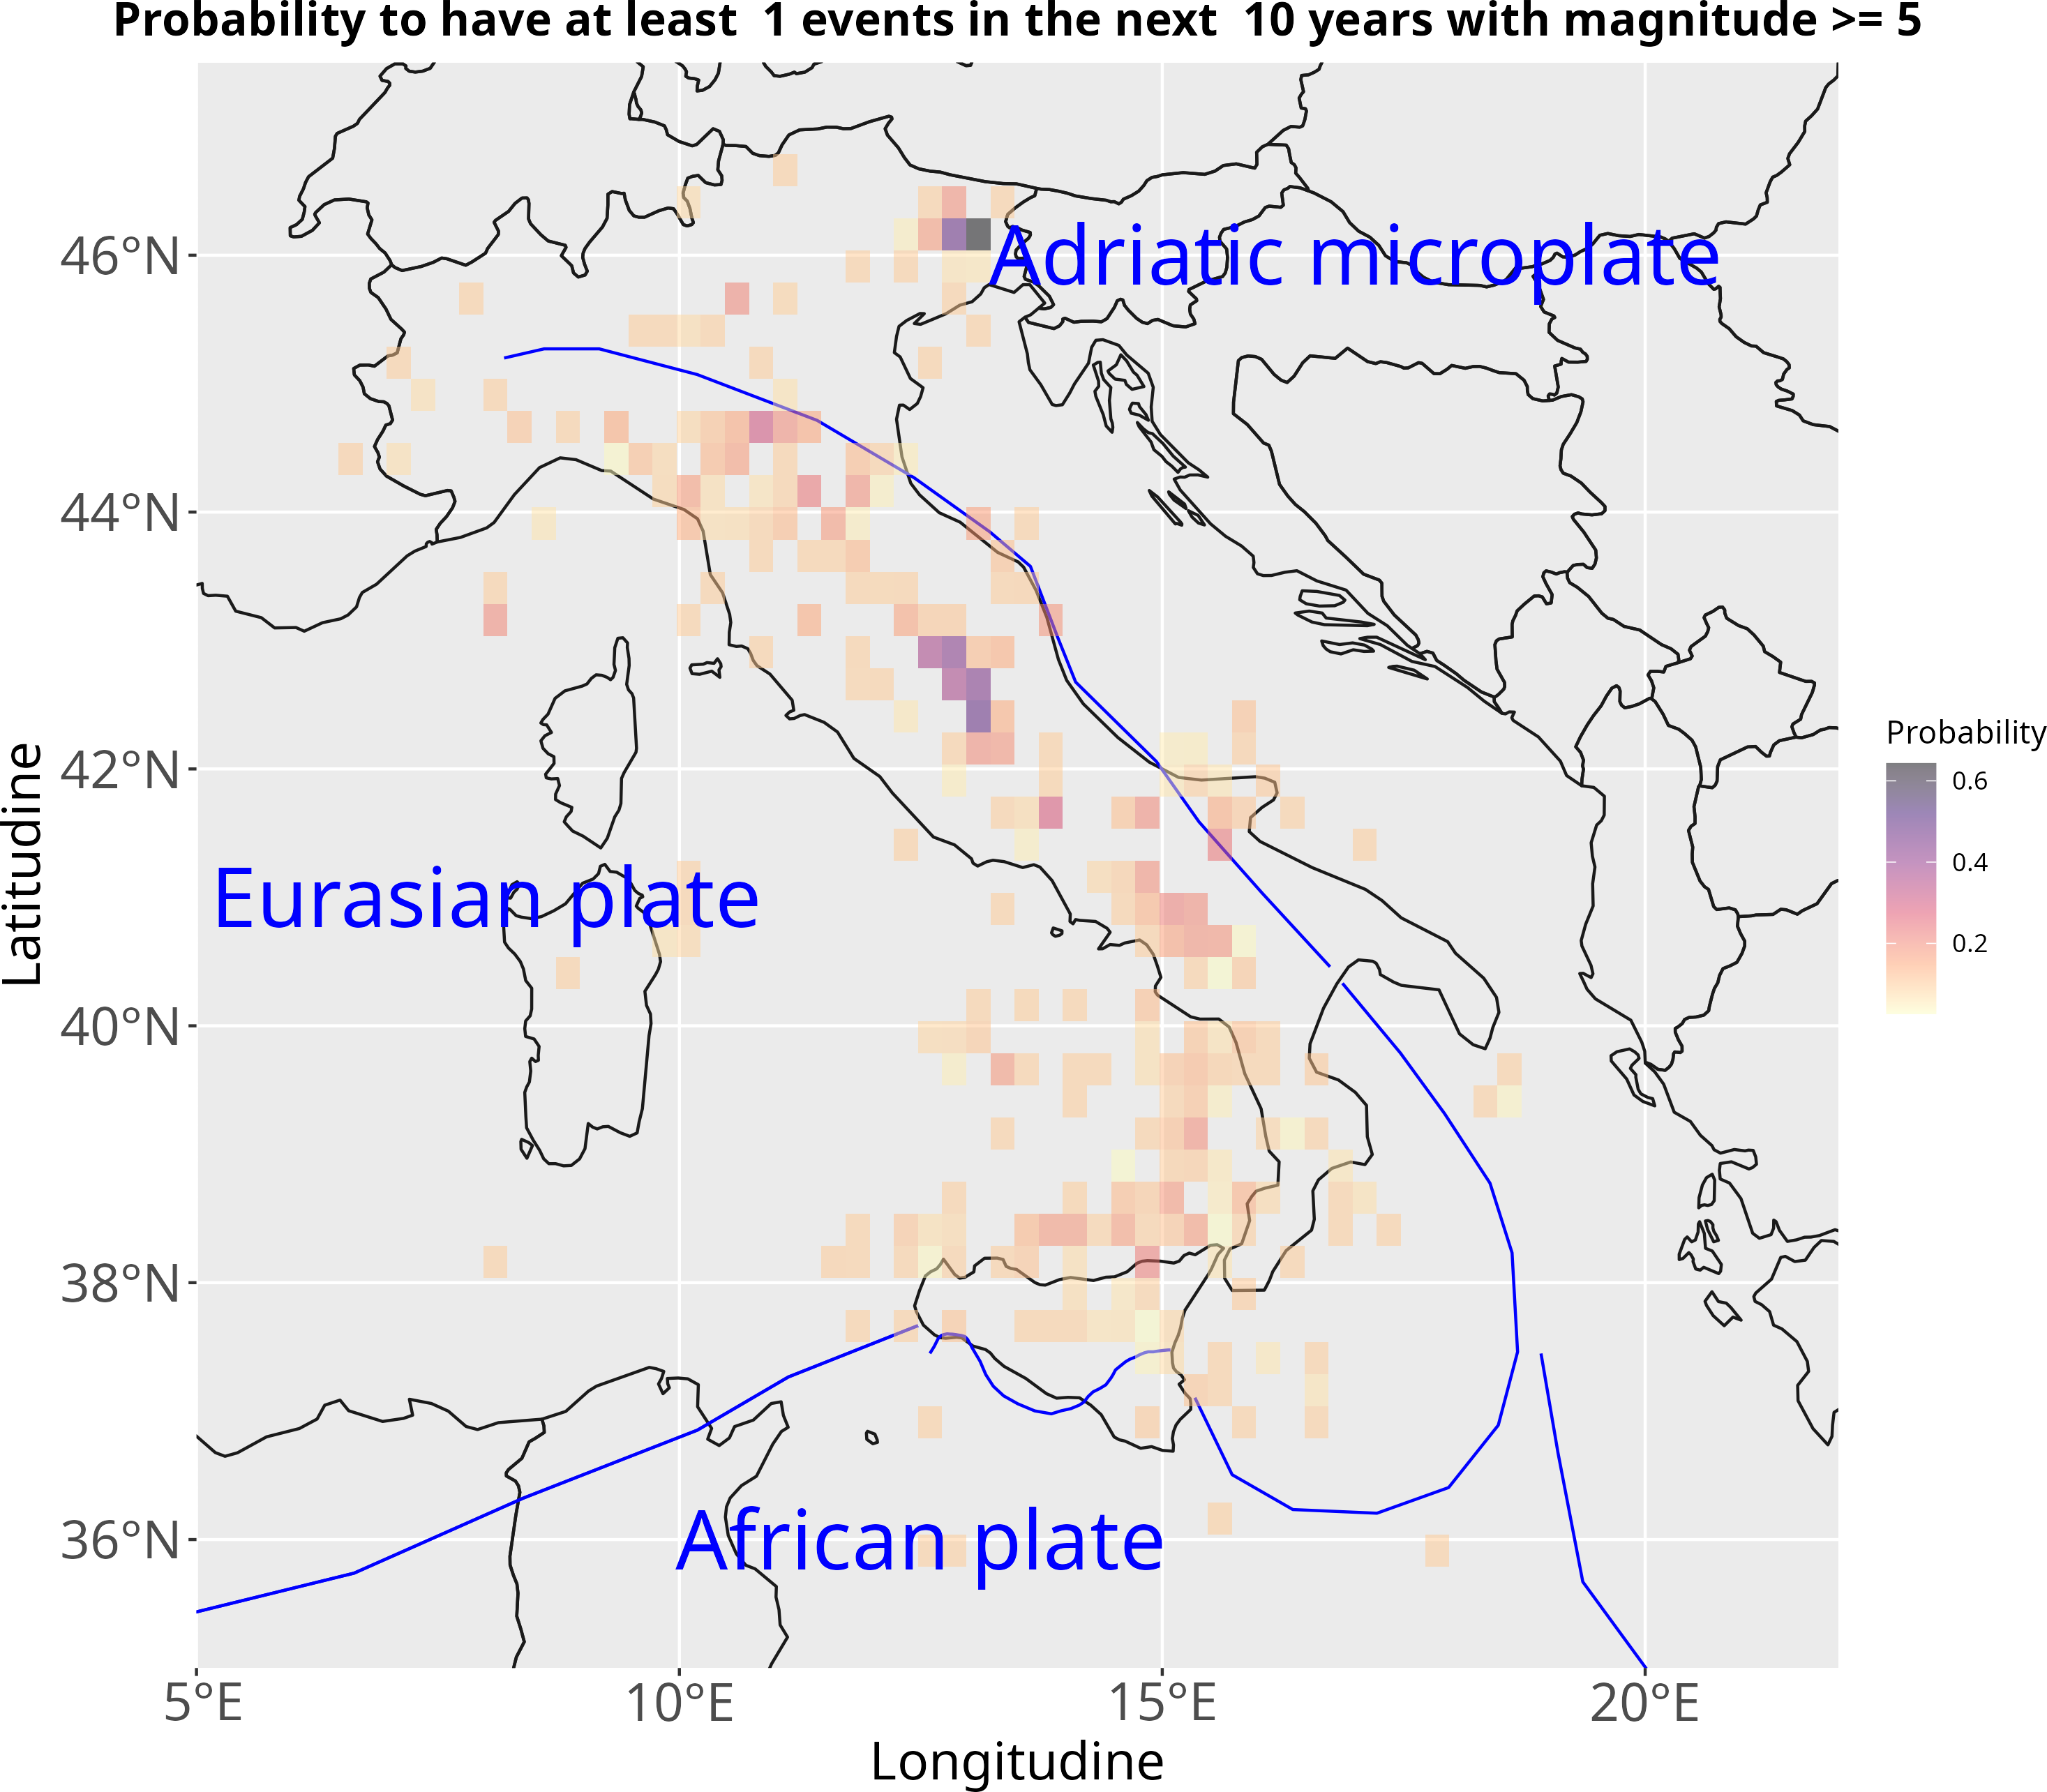
\includegraphics[width=0.85\textwidth]{EQ_images/probability.png} \\
\end{frame}

\begin{frame}{Hierarchical clustering}
	\centering
	\begin{minipage}{0.35\textwidth}
		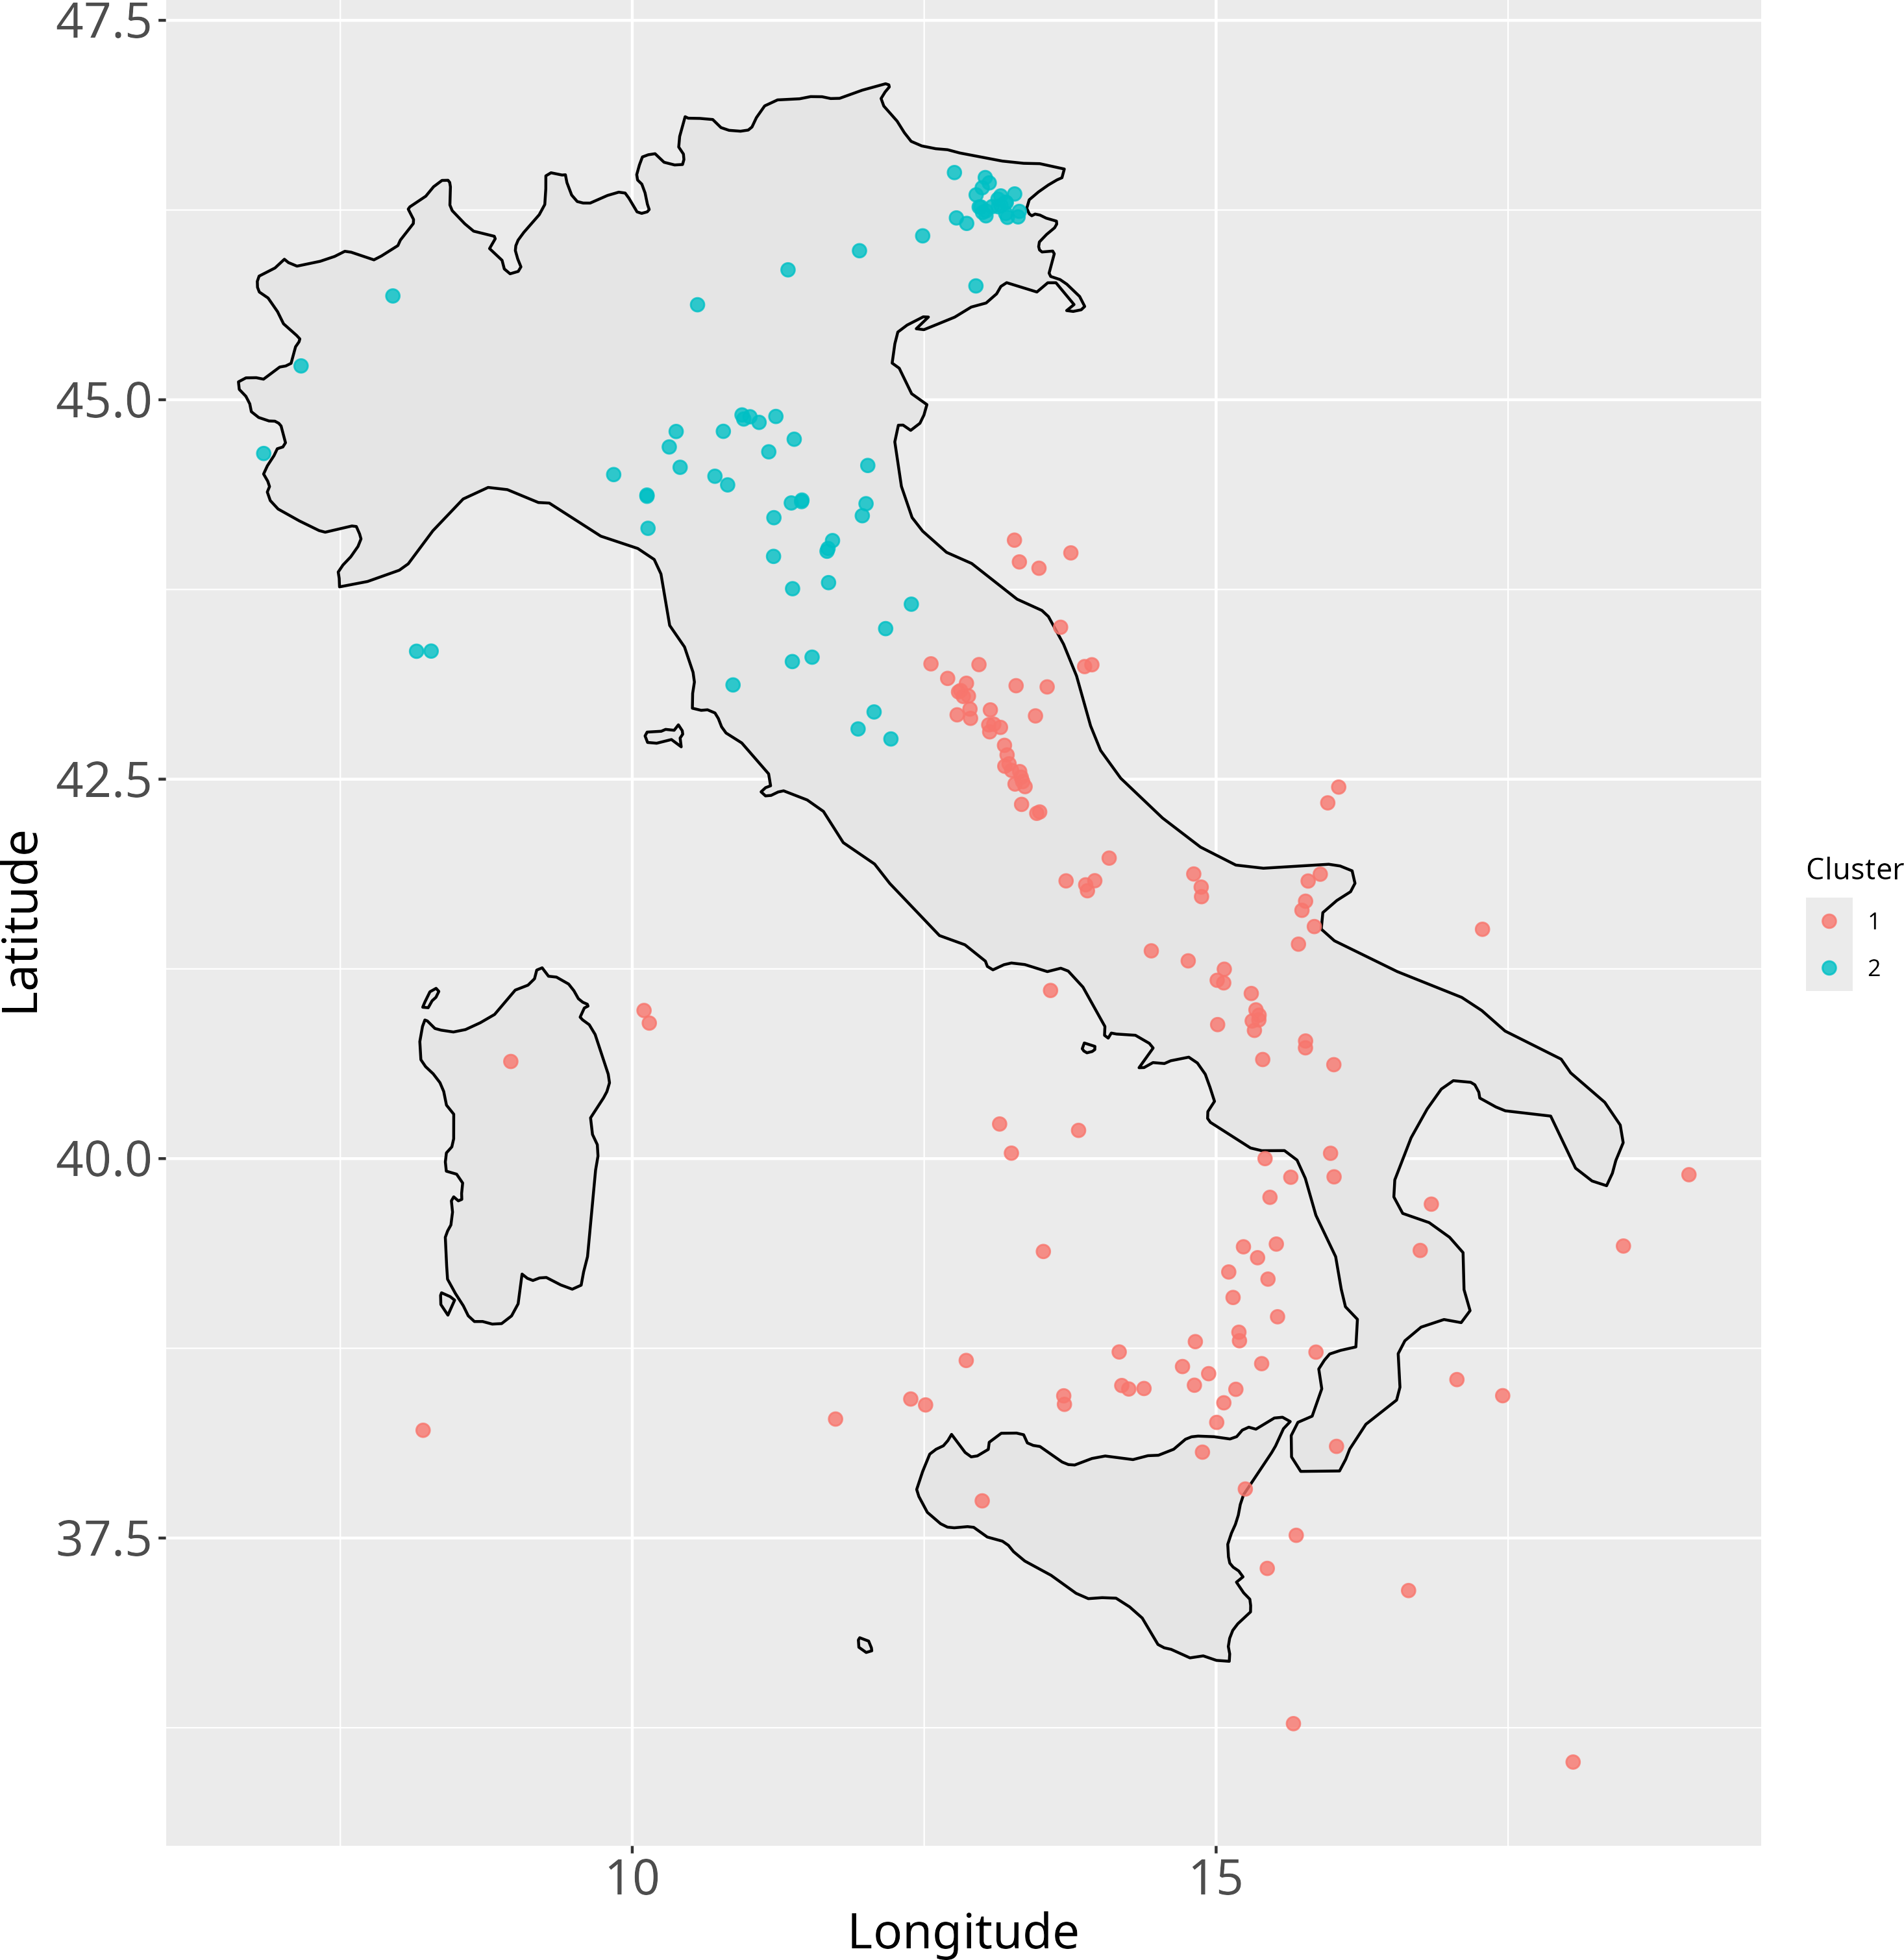
\includegraphics[width=\textwidth]{EQ_images/clustering_2.png}
	\end{minipage}
	\hspace{0.05\textwidth}
	\begin{minipage}{0.35\textwidth}
		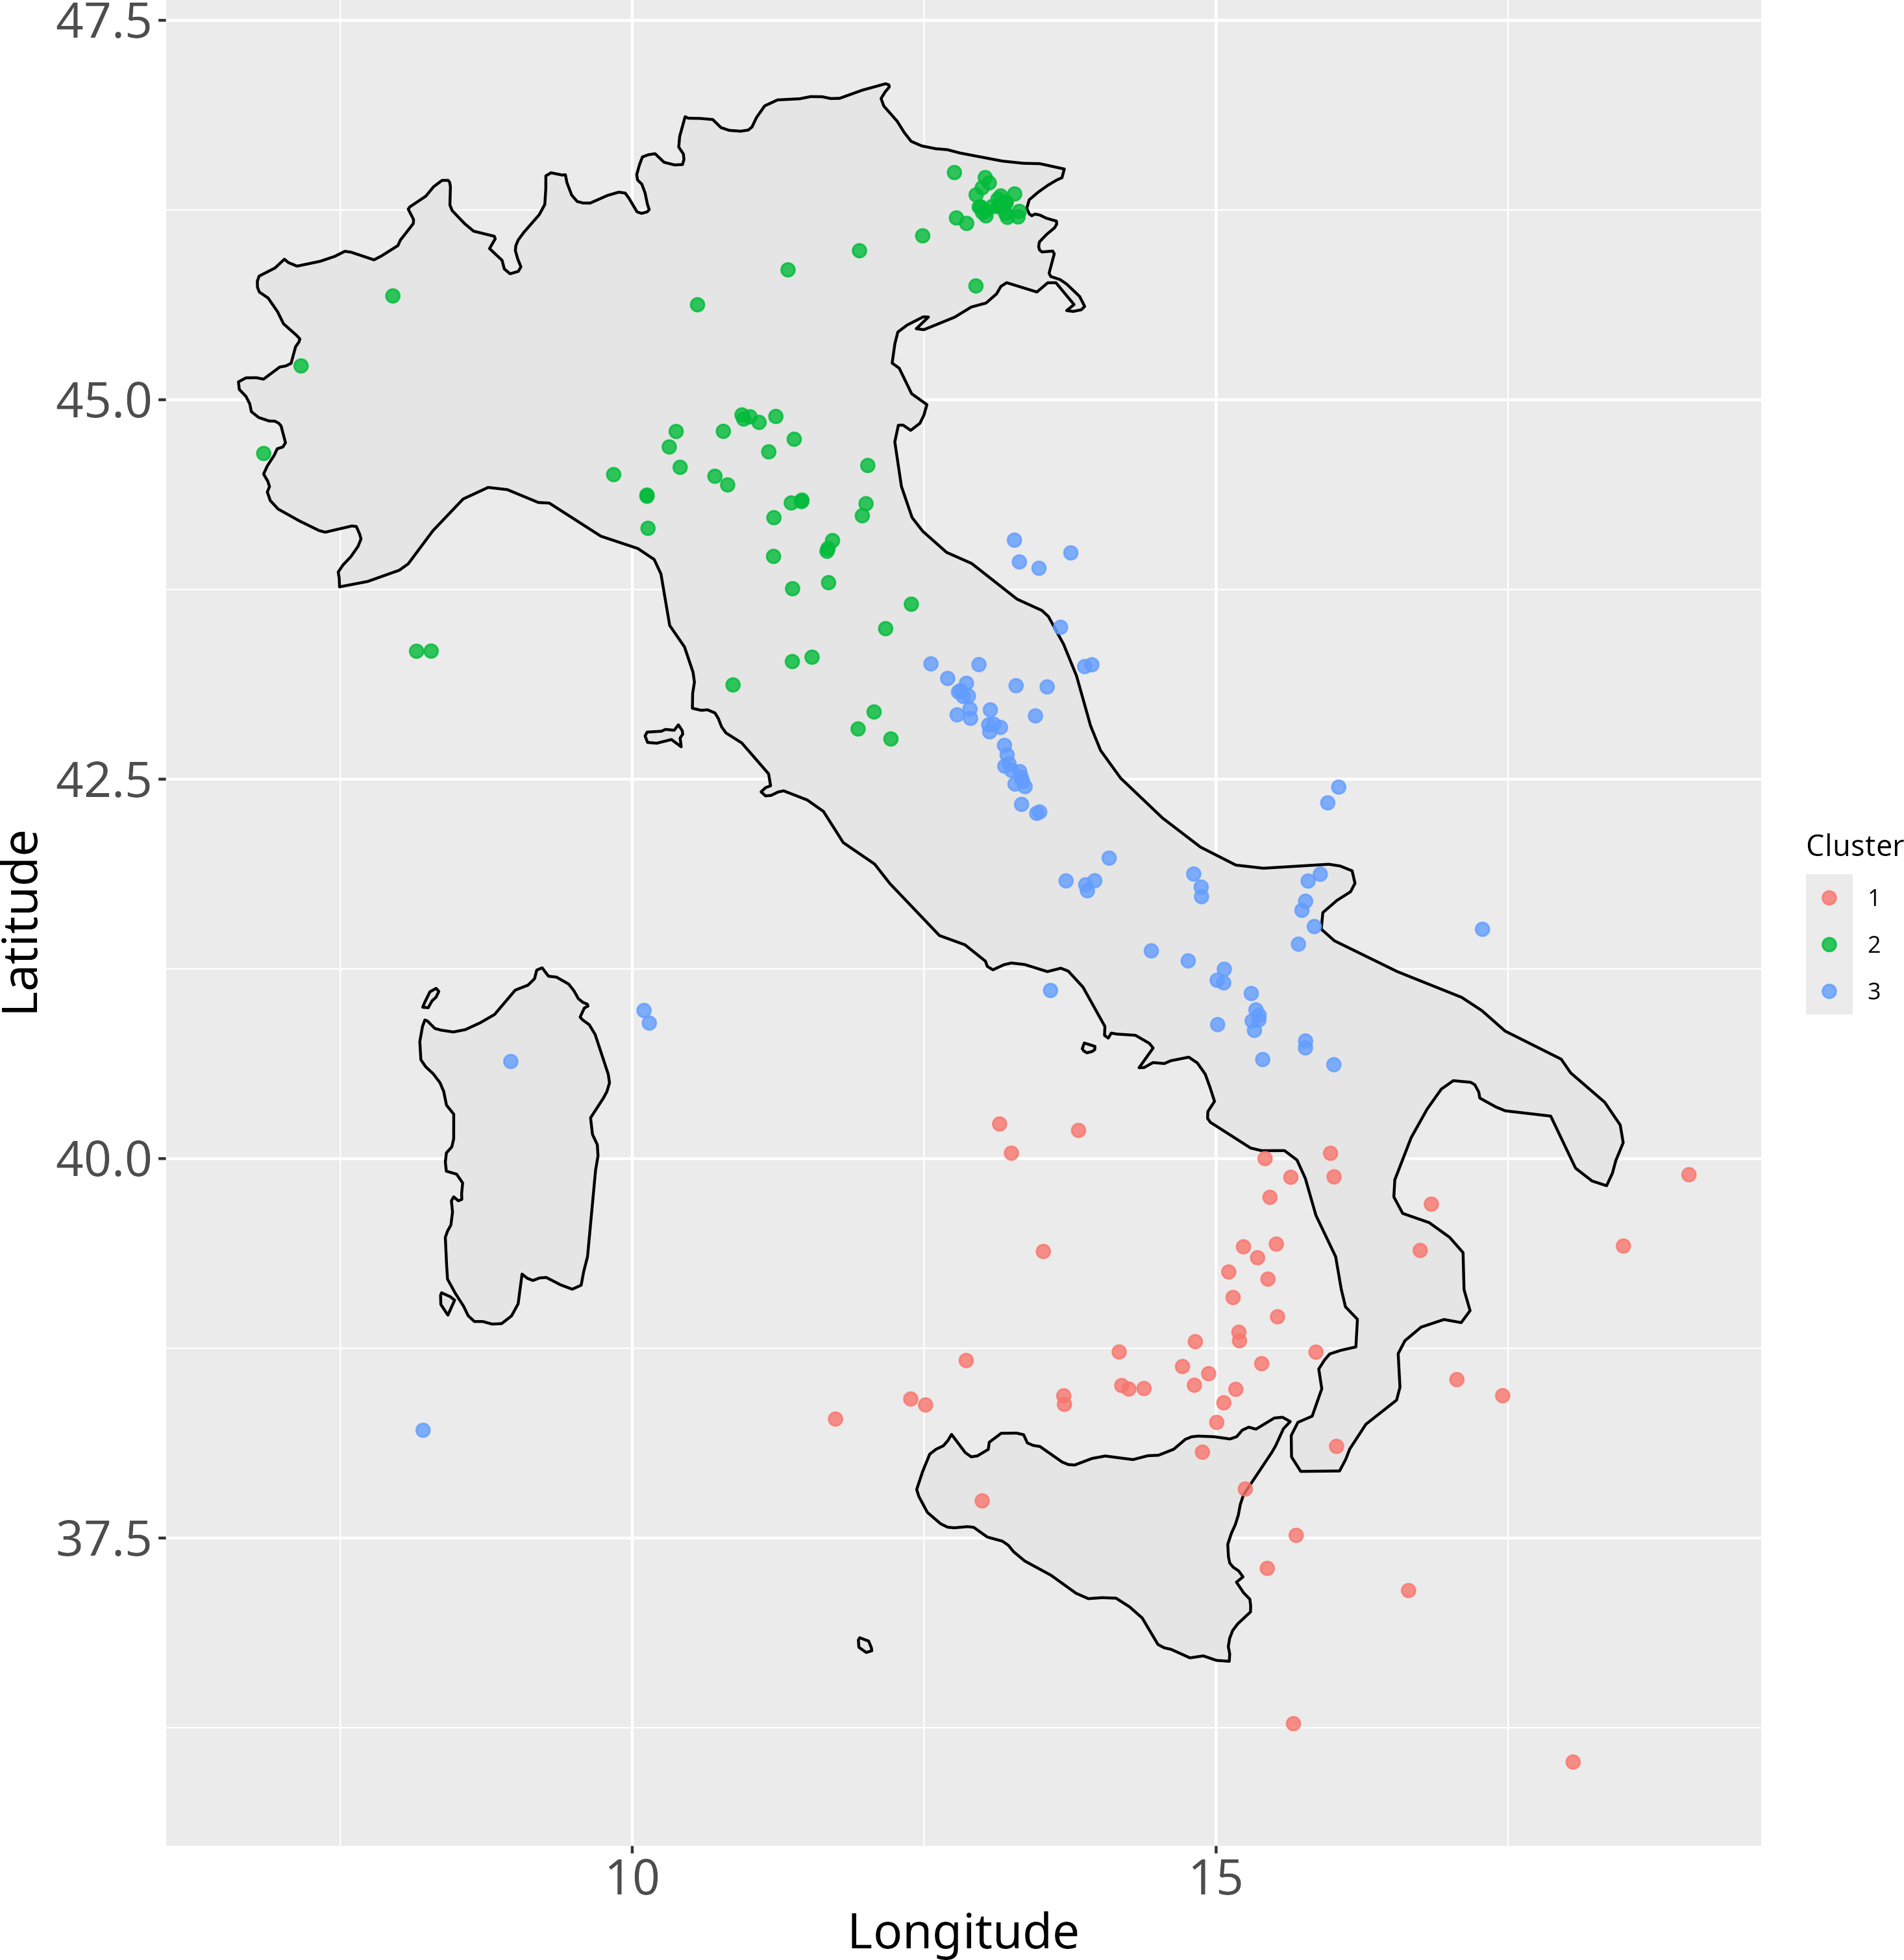
\includegraphics[width=\textwidth]{EQ_images/clustering_3.png}
	\end{minipage}
	
	\vspace{0.25cm}
	
	\begin{minipage}{0.35\textwidth}
		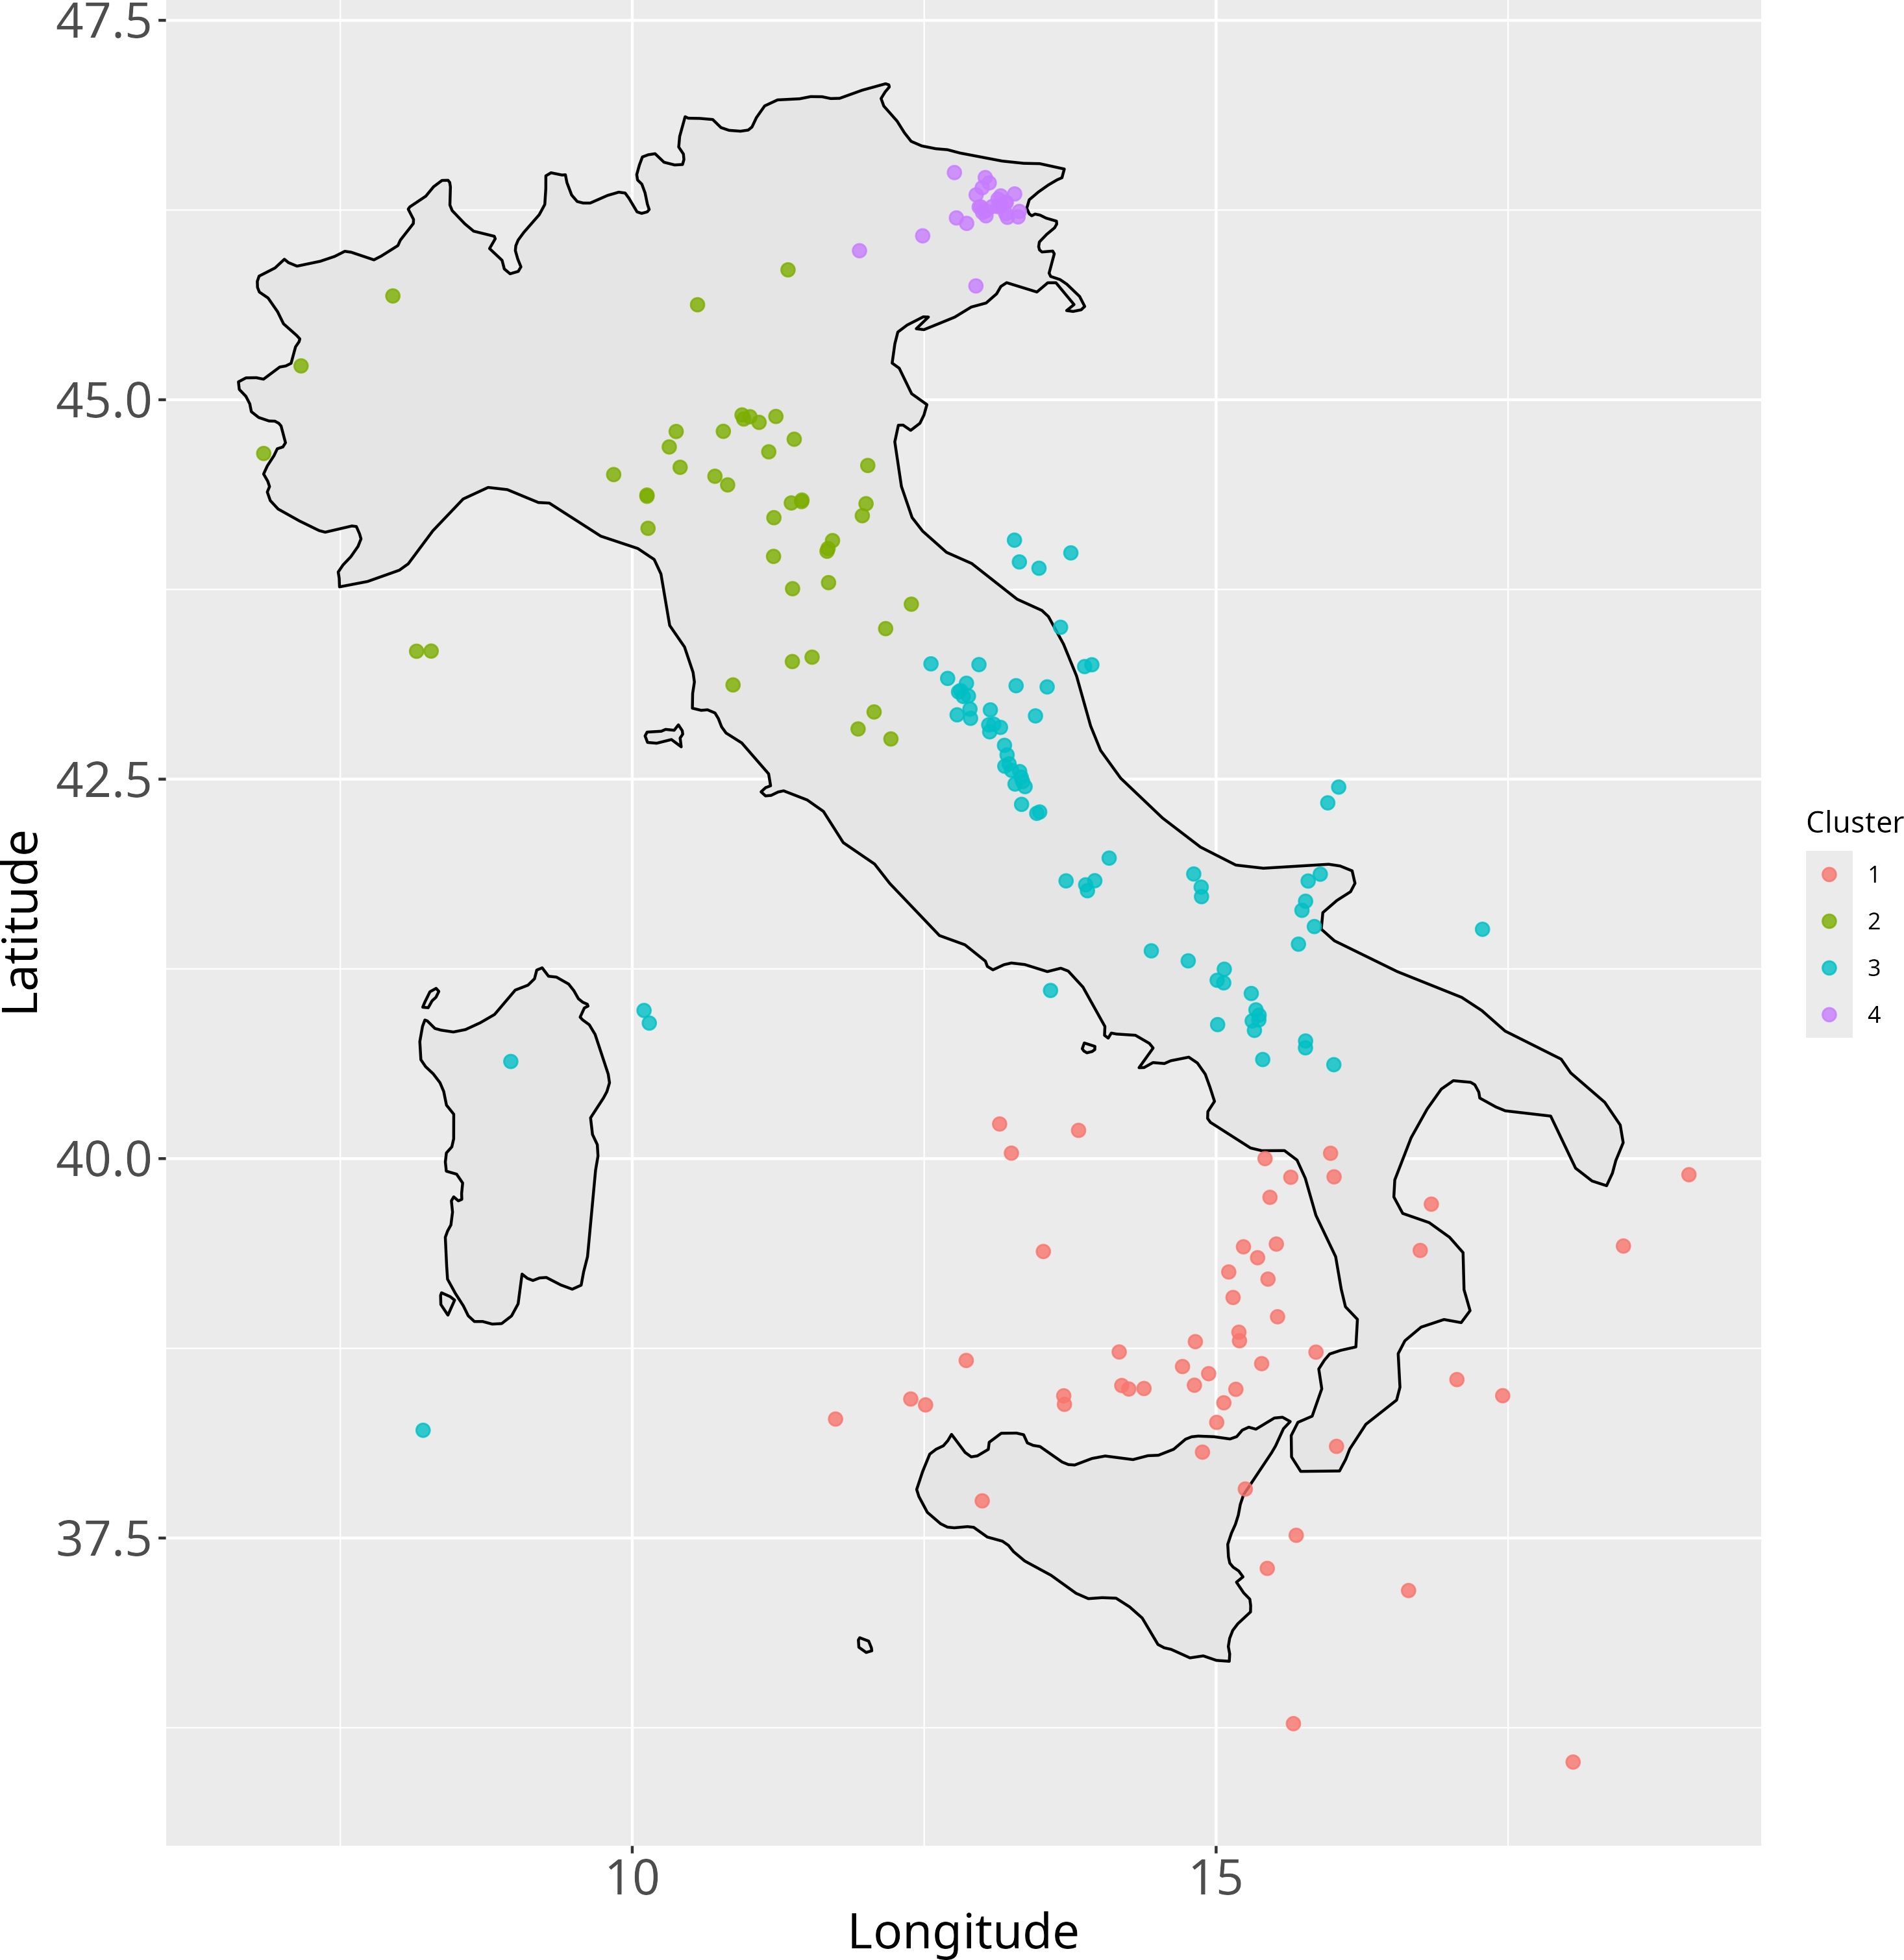
\includegraphics[width=\textwidth]{EQ_images/clustering_4.png}
	\end{minipage}
	\hspace{0.05\textwidth}
	\begin{minipage}{0.35\textwidth}
		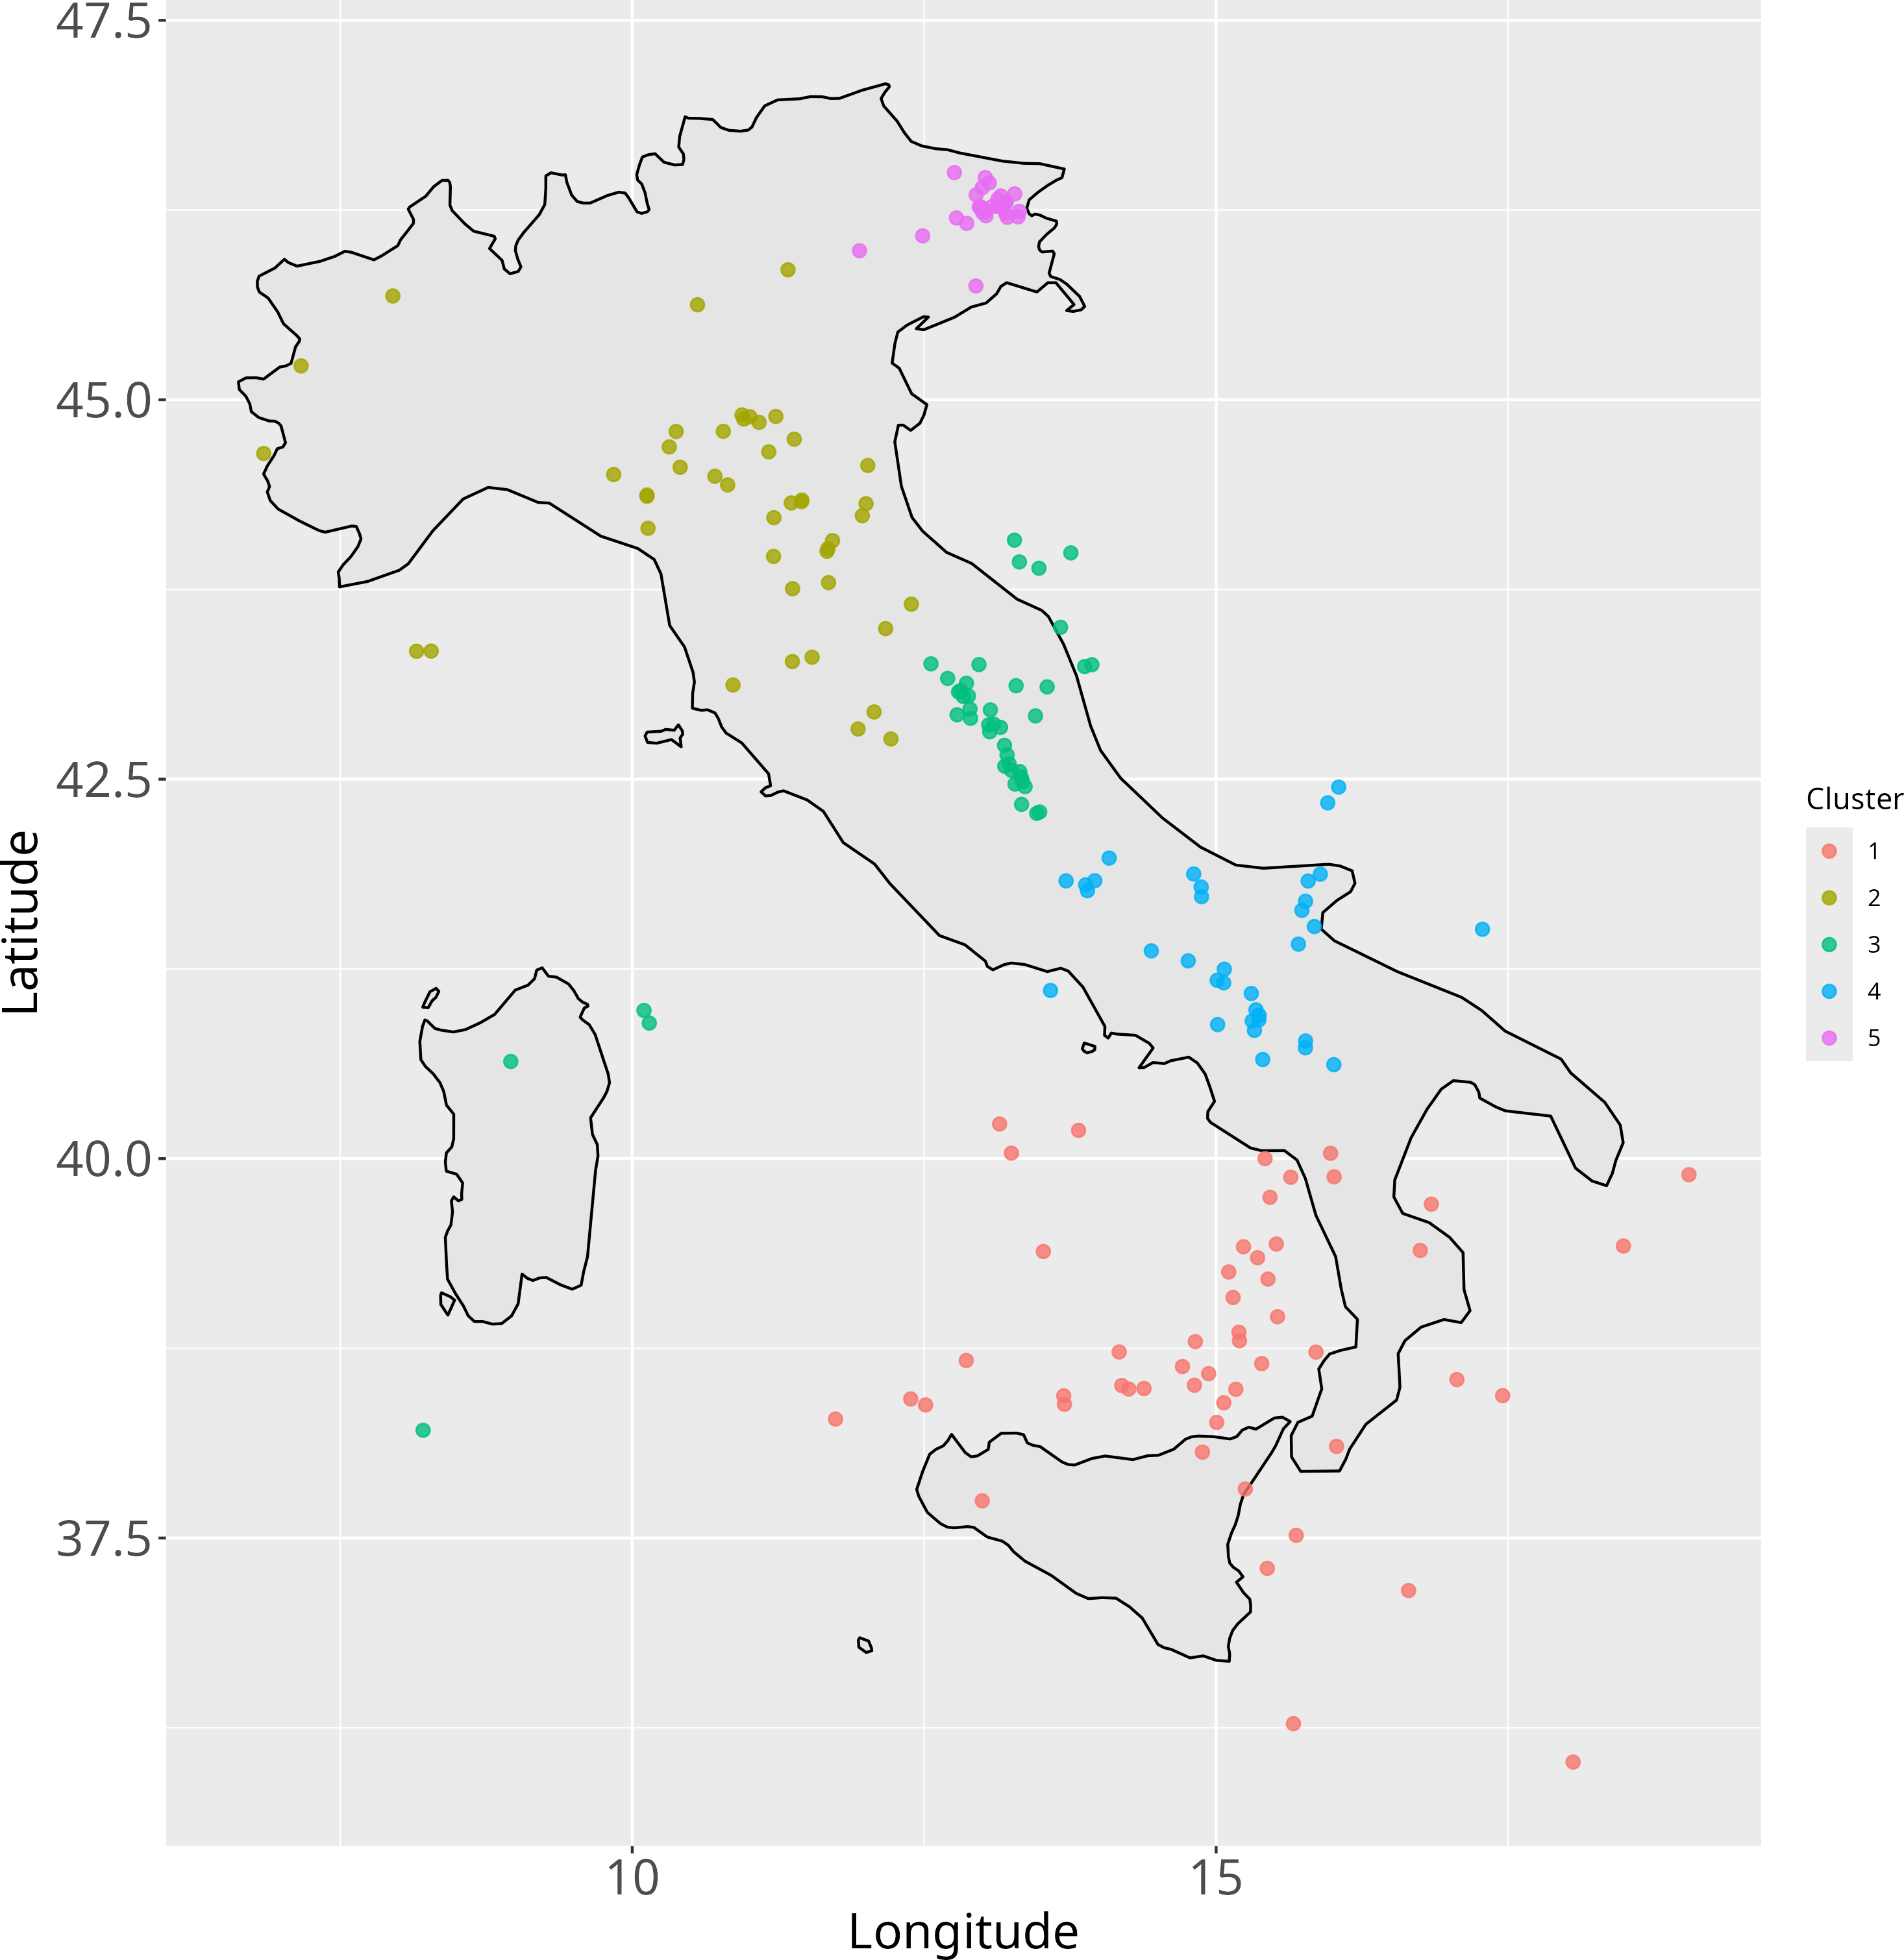
\includegraphics[width=\textwidth]{EQ_images/clustering_5.png}
	\end{minipage}
\end{frame}



\section{Third Part}




\begin{emptyframe}
	Thanks for your attention!
\end{emptyframe}


\end{document}


